%%%%%%%%%%%%%%%%%%%%%%%%%%%%%%%%%%%%%%%%%%%%%%%%%%%%%%%%%%%%%%%%%%%%%%%%
% Escuela Politécnica Superior de la Universidad de Alicante
% Realizado por: Jose Manuel Requena Plens
% Contacto: info@jmrplens.com / Telegram:@jmrplens
%%%%%%%%%%%%%%%%%%%%%%%%%%%%%%%%%%%%%%%%%%%%%%%%%%%%%%%%%%%%%%%%%%%%%%%%

\definecolor{mycolor1}{rgb}{1.00000,0.00000,1.00000}%
%
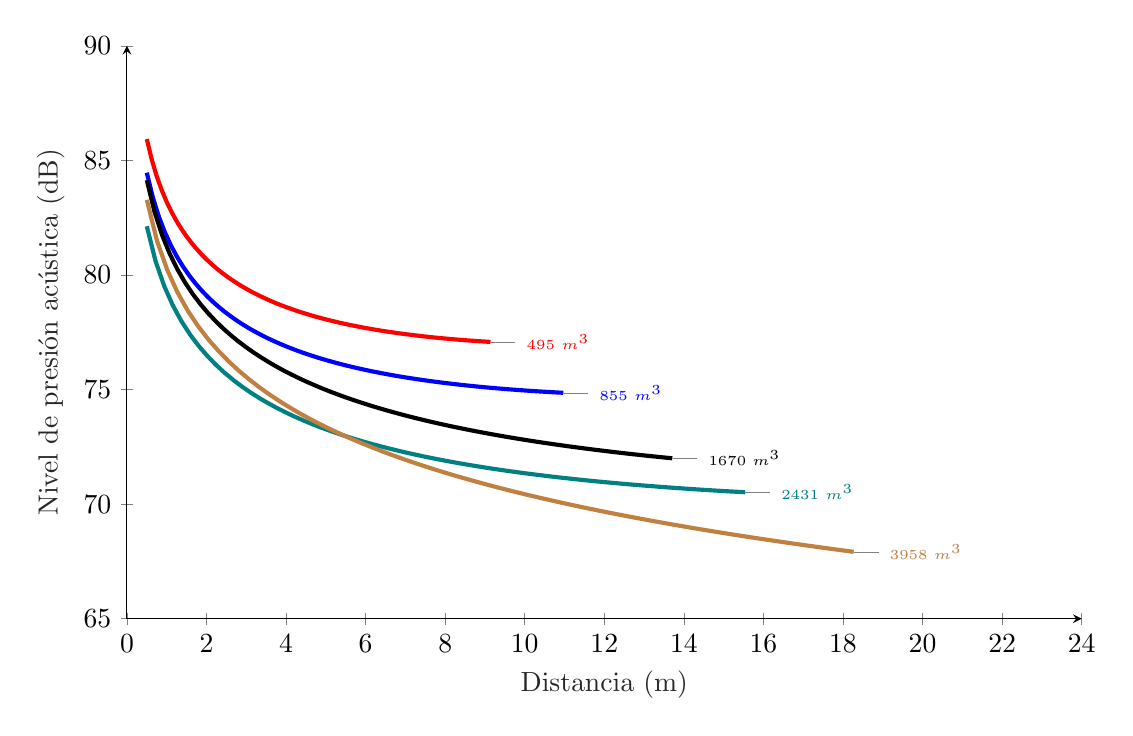
\begin{tikzpicture}

\begin{axis}[%
width=\textwidth,
height=0.6\textwidth,
at={(0\textwidth,0\textwidth)},
scale only axis,
xmin=0,
xmax=24,
xlabel style={font=\color{white!15!black}},
xlabel={Distancia (m)},
ymin=65,
ymax=90,
axis y line=left,
axis x line=bottom,
cycle list name=color list,
ylabel style={font=\color{white!15!black}},
ylabel={Nivel de presión acústica (dB)},
axis background/.style={fill=white},
legend style={legend cell align=left, align=left, draw=white!15!black}
]

% Capos utiles

% 1
\addplot+[ line width=1.5,domain=0.5:9.14, samples=70,every node/.style={xshift=-4pt}]
{10*log10(1.0337e+12 * ( ( 4*0.0026389378 / (512*(-ln(1-0.1176))*x) * ( e^(-(13.82*(x/343)*(-2.123) / 1.24))*1.683 - e^(-(13.82*((x/343)+0.05)*1.195 / 1.24))*1.175))))} node [pos=1,pin=0:{\tiny{495 $m^3$}}] {};

% 1.2
\addplot+[ line width=1.5,domain=0.5:10.97, samples=70,every node/.style={xshift=-4pt}]
{10*log10(1.0337e+12 * (  ( 4*0.0026389378 / (737*(-ln(1-0.1176))*x) * ( e^(-(13.82*(x/343)*(-2.095) / 1.49))*1.756 - e^(-(13.82*((x/343)+0.05)*1.309 / 1.49))*1.168))))} node [pos=1,pin=0:{\tiny{855 $m^3$}}] {};

% 1.5
\addplot+[ line width=1.5,domain=0.5:13.71, samples=70,every node/.style={xshift=-4pt}]
{10*log10(1.0337e+12 * (  ( 4*0.0026389378 / (1152*(-ln(1-0.1176))*x) * ( e^(-(13.82*(x/343)*(-1.176) / 1.86))*2.334 - e^(-(13.82*((x/343)+0.05)*1.373 / 1.86))*1.101))))} node [pos=1,pin=0:{\tiny{1670 $m^3$}}] {};

%% 1.7
\addplot[line width=1.5,color=teal, domain=0.5:15.54, samples=70,every node/.style={xshift=-4pt}]
{10*log10(1.0337e+12 * ( ( 4*0.0026389378 / (1479*(-ln(1-0.1176))*x) * ( e^(-(13.82*(x/343)*(-1.776) / 2.11))*2.014 - e^(-(13.82*((x/343)+0.05)*1.422 / 2.11))*1.074))))} node [pos=1,pin=0:{\tiny{2431 $m^3$}}] {};

% 20
\addplot+[ line width=1.5,domain=0.5:18.27, samples=70,every node/.style={xshift=-4pt}]
{10*log10(1.0337e+12 * ( ( 4*0.0026389378 / (2048*(-ln(1-0.1176))*x) * ( e^(-(13.82*(x/343)*0.087 / 2.49))*3.182 - e^(-(13.82*((x/343)+0.05)*1.486 / 2.49))*1.045))))} node [pos=1,pin=0:{\tiny{3958 $m^3$}}] {};

% 20
%\addplot+[ domain=0.5:23.88, samples=70,every node/.style={xshift=-4pt}]
%{10*log10(1.0337e+12 * ( ( 4*0.0026389378 / (\S*(-ln(1-0.1176))*x) * ( e^(-(13.82*(x/343)*\epsilonE / \T))*\CE - e^(-(13.82*((x/343)+0.05)*\epsilonL / \T))*\CL))))} node [pos=0.75,pin=15:{$\epsilon_E=-2$}] {};

\end{axis}
\end{tikzpicture}%



